\documentclass{beamer}\usepackage[]{graphicx}\usepackage[]{color}
% maxwidth is the original width if it is less than linewidth
% otherwise use linewidth (to make sure the graphics do not exceed the margin)
\makeatletter
\def\maxwidth{ %
  \ifdim\Gin@nat@width>\linewidth
    \linewidth
  \else
    \Gin@nat@width
  \fi
}
\makeatother

\definecolor{fgcolor}{rgb}{0.345, 0.345, 0.345}
\newcommand{\hlnum}[1]{\textcolor[rgb]{0.686,0.059,0.569}{#1}}%
\newcommand{\hlstr}[1]{\textcolor[rgb]{0.192,0.494,0.8}{#1}}%
\newcommand{\hlcom}[1]{\textcolor[rgb]{0.678,0.584,0.686}{\textit{#1}}}%
\newcommand{\hlopt}[1]{\textcolor[rgb]{0,0,0}{#1}}%
\newcommand{\hlstd}[1]{\textcolor[rgb]{0.345,0.345,0.345}{#1}}%
\newcommand{\hlkwa}[1]{\textcolor[rgb]{0.161,0.373,0.58}{\textbf{#1}}}%
\newcommand{\hlkwb}[1]{\textcolor[rgb]{0.69,0.353,0.396}{#1}}%
\newcommand{\hlkwc}[1]{\textcolor[rgb]{0.333,0.667,0.333}{#1}}%
\newcommand{\hlkwd}[1]{\textcolor[rgb]{0.737,0.353,0.396}{\textbf{#1}}}%
\let\hlipl\hlkwb

\usepackage{framed}
\makeatletter
\newenvironment{kframe}{%
 \def\at@end@of@kframe{}%
 \ifinner\ifhmode%
  \def\at@end@of@kframe{\end{minipage}}%
  \begin{minipage}{\columnwidth}%
 \fi\fi%
 \def\FrameCommand##1{\hskip\@totalleftmargin \hskip-\fboxsep
 \colorbox{shadecolor}{##1}\hskip-\fboxsep
     % There is no \\@totalrightmargin, so:
     \hskip-\linewidth \hskip-\@totalleftmargin \hskip\columnwidth}%
 \MakeFramed {\advance\hsize-\width
   \@totalleftmargin\z@ \linewidth\hsize
   \@setminipage}}%
 {\par\unskip\endMakeFramed%
 \at@end@of@kframe}
\makeatother

\definecolor{shadecolor}{rgb}{.97, .97, .97}
\definecolor{messagecolor}{rgb}{0, 0, 0}
\definecolor{warningcolor}{rgb}{1, 0, 1}
\definecolor{errorcolor}{rgb}{1, 0, 0}
\newenvironment{knitrout}{}{} % an empty environment to be redefined in TeX

\usepackage{alltt}
\usetheme{Boadilla}

\makeatother
\setbeamertemplate{footline}
{
    \leavevmode%
    \hbox{%
    \begin{beamercolorbox}[wd=.4\paperwidth,ht=2.25ex,dp=1ex,center]{author in head/foot}%
        \usebeamerfont{author in head/foot}\insertshortauthor
    \end{beamercolorbox}%
    \begin{beamercolorbox}[wd=.55\paperwidth,ht=2.25ex,dp=1ex,center]{title in head/foot}%
        \usebeamerfont{title in head/foot}\insertshorttitle
    \end{beamercolorbox}%
    \begin{beamercolorbox}[wd=.05\paperwidth,ht=2.25ex,dp=1ex,center]{date in head/foot}%
        \insertframenumber{}
    \end{beamercolorbox}}%
    \vskip0pt%
}
\makeatletter
\setbeamertemplate{navigation symbols}{}

\usepackage[T1]{fontenc}
\usepackage{lmodern}
\usepackage{amssymb,amsmath,bm,bbm}
\renewcommand{\familydefault}{\sfdefault}

\usepackage{mathtools}
\usepackage{graphicx}
\usepackage{threeparttable}
\usepackage{booktabs}
\usepackage{siunitx}
\sisetup{parse-numbers=false}

\setlength{\OuterFrameSep}{-2pt}
\makeatletter
\preto{\@verbatim}{\topsep=-10pt \partopsep=-10pt }
\makeatother

\title[Week 10:\ Mixed Logit Model]{Week 10:\ Mixed Logit Model}
\author[ResEcon 703:\ Advanced Econometrics]{ResEcon 703:\ Topics in Advanced Econometrics}
\date{Matt Woerman\\University of Massachusetts Amherst}
\IfFileExists{upquote.sty}{\usepackage{upquote}}{}
\begin{document}


{\setbeamertemplate{footline}{} 
\begin{frame}[noframenumbering]
    \titlepage
\end{frame}
}

\begin{frame}\frametitle{Agenda}
    Last week
    \begin{itemize}
        \item Generalized extreme value models
    \end{itemize}
    \vspace{2ex}
    This week
    \begin{itemize}
    	\item \hyperlink{page.\getpagerefnumber{overview}}{Mixed logit model overview}
    	\item \hyperlink{page.\getpagerefnumber{prob}}{Mixed logit choice probabilities}
        \item \hyperlink{page.\getpagerefnumber{random}}{Random coefficients}
        \item \hyperlink{page.\getpagerefnumber{subs}}{Substitution patterns}
        \item \hyperlink{page.\getpagerefnumber{panel}}{Panel data}
        \item \hyperlink{page.\getpagerefnumber{empirical}}{Empirical considerations}
        \item \hyperlink{page.\getpagerefnumber{example}}{Mixed logit R example}
    \end{itemize}
    \vspace{2ex}
    This week's reading
    \begin{itemize}
    	\item Train textbook, chapter 6
    \end{itemize}
\end{frame}

\section{Mixed Logit Model Overview}
\label{overview}
\begin{frame}\frametitle{}
    \vfill
    \centering
    \begin{beamercolorbox}[center]{title}
        \Large Mixed Logit Model Overview
    \end{beamercolorbox}
    \vfill
\end{frame}

\begin{frame}\frametitle{Discrete Choice Models Recap}
    Logit model
    \begin{itemize}
        \item Strong assumption that unobserved components of utility are i.i.d.
        \item Simple closed-form expressions for choice probabilities
        \item Preference variation can only be represented by observed data
        \item Panel data applications are limited by the i.i.d. assumption
    \end{itemize}
    \vspace{2ex}
    Nested logit model (and other generalized extreme value models)
    \begin{itemize}
        \item Correlation between unobserved components of utility can be modeled
        \item Choice probabilities are more complex but still closed-form
        \item Preference variation can only be represented by observed data
        \item Panel data applications are limited by an i.i.d. assumption
    \end{itemize}
    \vspace{2ex}
    What if we want a richer representation of preference variation, more flexible substitution patterns, and an ability to use panel data?
    \begin{itemize}
        \item Mixed logit model!
    \end{itemize}
\end{frame}


\begin{frame}\frametitle{Mixed Logit Model}
    The mixed logit model overcomes three limitations of the logit model
    \begin{itemize}
        \item Unobserved (or random) preference variation
        \item Unrestricted substitution patterns
        \item Correlations in unobserved factors over time
    \end{itemize}
    \vspace{3ex}
    What is the catch?
    \begin{itemize}
        \item Mixed logit choice probabilities are not closed-form
        \item Estimation requires numerical simulation
    \end{itemize}
\end{frame}

\begin{frame}\frametitle{Mixed Logit Coefficients}
    How does the mixed logit model achieves this level of flexibility?
    \begin{itemize}
        \item It does not use a set of fixed coefficients for the entire population, $\bm{\beta}$
        \item It assumes there is a distribution of coefficients throughout the population, $f(\bm{\beta} \mid \bm{\theta})$
    \end{itemize}
    \vspace{3ex}
    Distributions of coefficients overcome the three main limitations of the logit model
    \begin{itemize}
        \item Model distributions of unobserved preferences among the sample of decision makers
        \item Impose correlations in unobserved utility among alternatives
        \item Represent individual preferences over time
    \end{itemize}
\end{frame}

\section{Mixed Logit Choice Probabilities}
\label{prob}
\begin{frame}\frametitle{}
    \vfill
    \centering
    \begin{beamercolorbox}[center]{title}
        \Large Mixed Logit Choice Probabilities
    \end{beamercolorbox}
    \vfill
\end{frame}

\begin{frame}\frametitle{Mixed Logit Choice Probabilities}
	Unlike the logit and nested logit models, the mixed logit model is not defined by an assumption about the joint density of unobserved utility, $\bm{\varepsilon}_n$ \\
	\vspace{3ex}
    A mixed logit model is any discrete choice model with choice probabilities of the form
    \begin{align*}
        P_{ni} & = \int L_{ni}(\bm{\beta}) f(\bm{\beta} \mid \bm{\theta}) d \bm{\beta} \\
        \intertext{where $L_{ni}(\bm{\beta})$ is the logit probability at a given set of coefficients, $\bm{\beta}$}
        L_{ni}(\bm{\beta}) & = \frac{e^{V_{ni}(\bm{\beta})}}{\sum_{j = 1}^J e^{V_{nj}(\bm{\beta})}}
    \end{align*}
    and $f(\bm{\beta} \mid \bm{\theta})$ is a density function of coefficients $\bm{\beta}$, which depends on a vector of parameters, $\bm{\theta}$
    \begin{itemize}
    	\item The mixed logit choice probability is not a closed-form expression
    \end{itemize}
\end{frame}

\begin{frame}\frametitle{Mixed Logit Choice Probabilities Intuition}
	\begin{align*}
        P_{ni} & = \int L_{ni}(\bm{\beta}) f(\bm{\beta} \mid \bm{\theta}) d \bm{\beta} \\
        L_{ni}(\bm{\beta}) & = \frac{e^{V_{ni}(\bm{\beta})}}{\sum_{j = 1}^J e^{V_{nj}(\bm{\beta})}}
    \end{align*} \\
	\vspace{3ex}
	The mixed logit choice probability is a weighted average of logit choice probabilities
	\begin{itemize}
		\item The logit choice probabilities are evaluated at different values of $\bm{\beta}$
		\item Each logit choice probability is weighted by the density $f(\bm{\beta} \mid \bm{\theta})$
	\end{itemize}
	\vspace{3ex}
	The mixed logit choice probability is a mixed function of logit choice probabilities, $L_{ni}(\bm{\beta})$, with the mixing distribution $f(\bm{\beta} \mid \bm{\theta})$
\end{frame}

\begin{frame}\frametitle{Distributions of Coefficients}
    We previously used the terms ``parameter'' and ``coefficient'' interchangeably, but we will use them to mean different things in the mixed logit model
    \begin{itemize}
        \item $\bm{\beta}$: Coefficients that appear in the utility expression
        \begin{itemize}
            \item We will not estimate these coefficients in the mixed logit model
            \item These coefficients are integrated out of the choice probability
        \end{itemize}
        \item $\bm{\theta}$: Parameters that define the density of random coefficients
        \begin{itemize}
            \item We will estimate these parameters in the mixed logit model
        \end{itemize}
    \end{itemize}
    \vspace{2ex}
    Some examples of distributions of coefficients that we can model
    \begin{itemize}
        \item Normal: $\bm{\beta} \sim \mathcal{N}(\bm{\mu}, \bm{\Sigma})$, we estimate $\bm{\theta} = \{\bm{\mu}, \bm{\Sigma}\}$
        \item Log-normal: $\ln \bm{\beta} \sim \mathcal{N}(\bm{\mu}, \bm{\Sigma})$, we estimate $\bm{\theta} = \{\bm{\mu}, \bm{\Sigma}\}$
        \item Uniform: $\bm{\beta} \sim \mathcal{U}(\bm{a}, \bm{b})$, we estimate $\bm{\theta} = \{\bm{a}, \bm{b}\}$
        \item Triangular: $\bm{\beta} \sim Tri(\bm{a}, \bm{b}, \bm{c})$, we estimate $\bm{\theta} = \{\bm{a}, \bm{b}, \bm{c}\}$
        \item Many other distributions to choose from
    \end{itemize}
\end{frame}

\section{Random Coefficients}
\label{random}
\begin{frame}\frametitle{}
    \vfill
    \centering
    \begin{beamercolorbox}[center]{title}
        \Large Random Coefficients
    \end{beamercolorbox}
    \vfill
\end{frame}

\begin{frame}\frametitle{Random Utility Model with Individual-Specific Coefficients}
	A common way to rationalize the mixed logit model is the random utility model with individual-specific coefficients \\
	\vspace{3ex}
    The utility that decision maker $n$ obtains from alternative $j$ is
    $$U_{nj} = \bm{\beta}_n' \bm{x}_{nj} + \varepsilon_{nj}$$ \\
    \begin{itemize}
        \item $\bm{x}_{nj}$: data for alternative $j$ and decision maker $n$
        \item $\bm{\beta}_n$: individual-specific vector of coefficients
        \item $\varepsilon_{nj}$: i.i.d.\ extreme value error term
    \end{itemize}
    \vspace{3ex}
    Each decision maker knows their own $\bm{\beta}_n$ and $\varepsilon_{nj}$, so the choice is deterministic from their perspective
    \begin{itemize}
        \item $n$ chooses $i$ if and only if $U_{ni} > U_{nj} ~\forall j \neq i$
    \end{itemize}
\end{frame}

\begin{frame}\frametitle{Random Utility Model with Random Coefficients}
	The utility that decision maker $n$ obtains from alternative $j$ is
    $$U_{nj} = \bm{\beta}_n' \bm{x}_{nj} + \varepsilon_{nj}$$
    But we (the researchers) do not observe $\bm{\beta}_n$ for any individual
    \begin{itemize}
    	\item We model $\bm{\beta}_n$ as a random variable with density $f(\bm{\beta} \mid \bm{\theta})$
    \end{itemize}
    \vspace{2ex}
    If we did know $\bm{\beta}_n$, then the model would be a standard logit with the \emph{conditional} choice probability
    $$L_{ni}(\bm{\beta}_n) = \frac{e^{\bm{\beta}_n' \bm{x}_{ni}}}{\sum_{j = 1}^J e^{\bm{\beta}_n' \bm{x}_{nj}}}$$
    But we do not know $\bm{\beta}_n$, so we have to integrate over the density of the random coefficients to obtain the \emph{unconditional} choice probability
    $$P_{ni} = \int \frac{e^{\bm{\beta}' \bm{x}_{ni}}}{\sum_{j = 1}^J e^{\bm{\beta}' \bm{x}_{nj}}} f(\bm{\beta} \mid \bm{\theta}) d \bm{\beta}$$
\end{frame}

\section{Substitution Patterns}
\label{subs}
\begin{frame}\frametitle{}
    \vfill
    \centering
    \begin{beamercolorbox}[center]{title}
        \Large Substitution Patterns
    \end{beamercolorbox}
    \vfill
\end{frame}

\begin{frame}\frametitle{Random Utility Model with Flexible Random Utility}
    Another common way to rationalize the mixed logit model is the random utility model with fully flexible correlations in random utilities \\
    \vspace{3ex}
    The utility that decision maker $n$ obtains from alternative $j$ is
    $$U_{nj} = \bm{\alpha}' \bm{x}_{nj} + \bm{\mu}_n' \bm{z}_{nj} + \varepsilon_{nj}$$ \\
    \begin{itemize}
        \item $\bm{x}_{nj}$, $\bm{z}_{nj}$: data for alternative $j$ and decision maker $n$
        \item $\bm{\alpha}$: vector of fixed coefficients
        \item $\bm{\mu}_n$: vector of random coefficients with mean zero
        \item $\varepsilon_{nj}$: i.i.d.\ extreme value error term
    \end{itemize}
    \vspace{3ex}
    We can combine the random components of utility into a single composite random utility term, $\eta_{nj}$
    $$\eta_{nj} = \bm{\mu}_n' \bm{z}_{nj} + \varepsilon_{nj}$$
\end{frame}

\begin{frame}\frametitle{Random Utility Model with Correlated Random Utility}
	The utility that decision maker $n$ obtains from alternative $j$ is
	\begin{align*}
		U_{nj} & = \bm{\alpha}' \bm{x}_{nj} + \eta_{nj}
		\intertext{where the random utility term, $\eta_{nj}$, is given by}
		\eta_{nj} & = \bm{\mu}_n' \bm{z}_{nj} + \varepsilon_{nj}
	\end{align*} \\
	\vspace{2ex}
	These flexible random utility terms can be correlated over alternatives
	$$Cov(\eta_{ni}, \eta_{nj}) = \bm{z}_{ni}' \bm{\Sigma} \bm{z}_{nj}$$
	where $\bm{\Sigma}$ is the variance-covariance matrix of $\bm{\mu}$ \\
	\vspace{2ex}
	The flexible specification of random utility yields flexible correlations between alternatives, which we can estimate
\end{frame}

\begin{frame}\frametitle{Special Cases of Correlated Random Utility}
    This representation of random utility correlations generalizes all of the previous discrete choice models we have discussed
    $$Cov(\eta_{ni}, \eta_{nj}) = \bm{z}_{ni}' \bm{\Sigma} \bm{z}_{nj}$$ \\
    \vspace{2ex}
    Logit model
    \begin{itemize}
    	\item When $z_{nj} = 0 ~\forall j$, the random utility of alternatives is uncorrelated
    \end{itemize}
    \vspace{2ex}
    Nested logit model
    \begin{itemize}
    	\item $\bm{z}_{nj}$ is a set of indicator variables for each nest
    	\begin{itemize}
    		\item $K$ variables that equal 1 for the alternatives in that nest
    	\end{itemize}
    	\item $\mu_k \sim \mathcal{N}(0, \sigma_k)$ and independent across nests
    	\item Covariance between alternatives in nest $k$ is $\sigma_k$, which we estimate
    \end{itemize}
\end{frame}

\begin{frame}\frametitle{Equivalence of Random Utility Models}
    We have motivated the mixed logit model from two random utility models
    \begin{itemize}
    	\item These random utility models are mathematically equivalent
    \end{itemize}
    \vspace{2ex}
    Starting from the random coefficients expression
    \begin{align*}
        U_{nj} & = \bm{\beta}_n' \bm{x}_{nj} + \varepsilon_{nj} \\
        \intertext{Express $\bm{\beta}_n$ as $\bm{\beta}_n = \bm{\alpha} + \bm{\mu}_n$ by decomposing $\bm{\beta}_n$ into the means, $\bm{\alpha}$, and the deviations from the means, $\bm{\mu}_n$}
        U_{nj} & = \bm{\alpha}' \bm{x}_{nj} + \bm{\mu}_n' \bm{z}_{nj} + \varepsilon_{nj}
    \end{align*}
    where $\bm{z}_{nj}$ is the subset of data, $\bm{x}_{nj}$, with random coefficients
    \begin{itemize}
    	\item If all variables have random coefficients, then $\bm{z}_{nj} = \bm{x}_{nj}$
    \end{itemize}
    \vspace{2ex}
    Your motivation will affect which coefficients you model as random and whether to allow correlations between the coefficients
\end{frame}

\begin{frame}\frametitle{Mixed Logit Substitution Patterns}
    If representative utility is linear, $V_{nj} = \bm{\beta}_n' \bm{x}_{nj}$, then the ratio of the choice probabilities of alternative $i$ and alternative $m$ is 
    $$\frac{P_{ni}}{P_{nm}} = \frac{\displaystyle \int \frac{e^{\bm{\beta}' \bm{x}_{ni}}}{\sum_{j = 1}^J e^{\bm{\beta}' \bm{x}_{nj}}} f(\bm{\beta} \mid \bm{\theta}) d \bm{\beta}}{\displaystyle \int \frac{e^{\bm{\beta}' \bm{x}_{nm}}}{\sum_{j = 1}^J e^{\bm{\beta}' \bm{x}_{nj}}} f(\bm{\beta} \mid \bm{\theta}) d \bm{\beta}}$$ \\
    \begin{itemize}
    	\item Choice probability denominators are inside the integrals, so they cannot cancel as they did in previous models
    \end{itemize}
    \vspace{3ex}
    The ratio of any two choice probabilities depends on all alternatives
    \begin{itemize}
    	\item The mixed logit model does not exhibit independence of irrelevant alternatives (IIA)
    \end{itemize}
\end{frame}

\begin{frame}\frametitle{Mixed Logit Elasticities}
    The own elasticity of alternative $i$ with respect to its attribute $z_{ni}$ (where $z_{ni}$ is any element of $\bm{x}_{ni}$) is
    \begin{align*}
    	E_{iz_{ni}} & = \frac{z_{ni}}{P_{ni}} \int \beta_z L_{ni}(\bm{\beta}) [1 - L_{ni}(\bm{\beta})] f(\bm{\beta} \mid \bm{\theta}) d \bm{\beta}
    	\intertext{The cross elasticity of alternative $i$ with respect to attribute $z_{nj}$ of alternative $j$ (where $z_{nj}$ is any element of $\bm{x}_{nj}$) is}
    	E_{iz_{nj}} & = - \frac{z_{nj}}{P_{ni}} \int \beta_z L_{ni}(\bm{\beta}) L_{nj}(\bm{\beta}) f(\bm{\beta} \mid \bm{\theta}) d \bm{\beta}
    \end{align*}
    As with the mixed logit choice probabilities, mixed logit elasticities do not have closed-form expressions \\
    \vspace{3ex}
    These expressions depend on how $L_{ni}(\bm{\beta})$ varies and how $L_{ni}(\bm{\beta})$ and $L_{nj}(\bm{\beta})$ covary as you integrate over the density of $\bm{\beta}$, which is determined by which parameters you specify as random and whether they covary
\end{frame}

\section{Panel Data}
\label{panel}
\begin{frame}\frametitle{}
    \vfill
    \centering
    \begin{beamercolorbox}[center]{title}
        \Large Panel Data
    \end{beamercolorbox}
    \vfill
\end{frame}

\begin{frame}\frametitle{Mixed Logit and Panel Data}
    The structure of the mixed logit model allows for more flexibility in representing how a single decision maker makes multiple choices over time periods, so it provides a better model for most panel data settings
    \begin{itemize}
        \item In the logit and nested logit models, all unobserved factors that influence utility are represented by $\bm{\varepsilon}_{nt}$, which is i.i.d., so those models cannot accommodate correlations over time
        \item But the mixed logit model allows for unobserved preference variation through random coefficients, which yields correlations in utility over time for the same decision maker
    \end{itemize}
\end{frame}

\begin{frame}\frametitle{Mixed Logit Model with Panel Data}
    We add a time index, $t$, to our random utility model but assume the random coefficients, $\bm{\beta}_n$, are constant for an individual
    $$U_{njt} = \bm{\beta}_n' \bm{x}_{njt} + \varepsilon_{njt}$$
    and we consider the vector of alternatives that decision maker $n$ chooses over the $T$ time periods
    $$\bm{i} = (i_1, \ldots, i_T)$$
    Then the conditional logit probability for a sequence of choices is
    \begin{align*}
        L_{n\bm{i}}(\bm{\beta}) & = \prod_{t = 1}^T \frac{e^{\bm{\beta}' \bm{x}_{ni_{t}t}}}{\sum_{j = 1}^J e^{\bm{\beta}' \bm{x}_{njt}}} \\
        \intertext{and integrating over the density of coefficients gives the choice probability}
        P_{n\bm{i}} & = \int L_{n\bm{i}}(\bm{\beta}) f(\bm{\beta} \mid \bm{\theta}) d \bm{\beta}
    \end{align*}
\end{frame}

\begin{frame}\frametitle{Dynamics in a Mixed Logit Model}
    Some ``dynamics'' can be represented in a mixed logit model using panel data
    \begin{itemize}
        \item Past and future exogenous variables can be included to model lagged or anticipatory behavior
        \item Lagged dependent variables can be included to represent state dependence 
    \end{itemize}
    \vspace{3ex}
    This approach is a relatively naive way of incorporating dynamics into a discrete choice model
    \begin{itemize}
        \item We are essentially modeling a sequence of static choices
        \item A fully ``dynamic discrete choice model'' would model how every choice affects all subsequent choices
        \item We will talk about dynamic discrete choice models in the final week of the semester
    \end{itemize}
\end{frame}

\section{Empirical Considerations}
\label{empirical}
\begin{frame}\frametitle{}
    \vfill
    \centering 
    \begin{beamercolorbox}[center]{title}
        \Large Empirical Considerations
    \end{beamercolorbox}
    \vfill
\end{frame}

\begin{frame}\frametitle{Mixed Logit Estimation}
    Mixed logit choice probabilities do not have a closed-form expression
    $$P_{ni} = \int \frac{e^{\bm{\beta}' \bm{x}_{ni}}}{\sum_{j = 1}^J e^{\bm{\beta}' \bm{x}_{nj}}} f(\bm{\beta} \mid \bm{\theta}) d \bm{\beta}$$ \\
    \begin{itemize}
        \item We cannot estimate a mixed logit model using maximum likelihood because we cannot calculate the log-likelihood function
    \end{itemize}
    \vspace{2ex}
    Instead, we can approximate choice probabilities through numerical simulation, calculate the simulated log-likelihood function, and estimate using maximum simulated likelihood 
    \begin{itemize}
        \item More on other simulation-based estimation methods next week
    \end{itemize}
    \vspace{2ex}
    We can use the \texttt{mlogit()} function in R to estimate mixed logit models
    \begin{itemize}
        \item We specify our random coefficients using the \texttt{rpar} argument in the \texttt{mlogit()} function
    \end{itemize}
\end{frame}

\begin{frame}\frametitle{Mixed Logit with Market-Level Data}
    The mixed logit model can also be estimated from market-level data
    \begin{itemize}
        \item You observe the price, market share, and characteristics of every cereal brand at the grocery store, and you want to estimate the structural parameters of consumer decision making that explain those purchases
    \end{itemize}
    \vspace{2ex}
    When aggregated over many consumers, choice probabilities become market shares
    $$S_i = \int \frac{e^{\bm{\beta}' \bm{x}_i}}{\sum_{j = 1}^J e^{\bm{\beta}' \bm{x}_j}} f(\bm{\beta} \mid \bm{\theta}) d \bm{\beta}$$
    \begin{itemize}
        \item Because of the integral, mixed logit market shares do not reduce to a linear model as they did for logit and nested logit
        \item Demand estimation using random coefficients logit often uses the ``BLP'' method of Berry, Levinsohn, and Pakes (1995)
        \item We will talk about BLP in the final week of the semester
    \end{itemize}
\end{frame}

\section{Mixed Logit R Example}
\label{example}
\begin{frame}\frametitle{}
    \vfill
    \centering
    \begin{beamercolorbox}[center]{title}
        \Large Mixed Logit R Example
    \end{beamercolorbox}
    \vfill
\end{frame}

\begin{frame}\frametitle{Mixed Logit Model Example}
    We are again studying how consumers make choices about expensive and highly energy-consuming systems in their homes
    \begin{itemize}
    	\item We have (real) data on 250 households in California and the type of HVAC (heating, ventilation, and air conditioning) system in their home. Each household has the following choice set, and we observe the following data
    \end{itemize}
    \vspace{2ex}
    \begin{columns}
    	\begin{column}{0.5\textwidth}
		    Choice set
		    \begin{itemize}
		    	\item \texttt{ec}: electric central
		    	\item \texttt{ecc}: electric central with AC
		    	\item \texttt{er}: electric room
		    	\item \texttt{erc}: electric room with AC
		    	\item \texttt{gc}: gas central
		    	\item \texttt{gcc}: gas central with AC
		    	\item \texttt{hpc}: heat pump with AC
		    \end{itemize}
	    \end{column}
	    \begin{column}{0.5\textwidth}
		    Alternative-specific data
		    \begin{itemize}
		    	\item \texttt{ich}: installation cost for heat
		    	\item \texttt{icca}: installation cost for AC
		    	\item \texttt{och}: operating cost for heat
		    	\item \texttt{occa}: operating cost for AC
		    \end{itemize}
		    \vspace{2ex}
		    Household demographic data
		    \begin{itemize}
		    	\item \texttt{income}: annual income
		    \end{itemize}
		    \vspace{1ex}
		\end{column}
    \end{columns}
\end{frame}

\begin{frame}\frametitle{Random Utility Model of HVAC System Choice}
    We model the utility to household $n$ of installing HVAC system $j$ as
    $$U_{nj} = V_{nj} + \varepsilon_{nj}$$
    where $V_{nj}$ depends on the data about alternative $j$ and household $n$ \\
    \vspace{3ex}
    The probability that household $n$ installs HVAC system $i$ is
 	$$P_{ni} = \int_{\bm{\varepsilon}} \mathbbm{1}(\varepsilon_{nj} - \varepsilon_{ni} < V_{ni} - V_{nj} \; \forall j \neq i) f(\bm{\varepsilon}_n) d\bm{\varepsilon}_n$$ \\
 	\vspace{2ex}
  	Under the logit assumption, these choice probabilities simplify to
    $$P_{ni} = \frac{e^{V_{ni}}}{\sum_j e^{V_{nj}}}$$
\end{frame}

\begin{frame}\frametitle{Representative Utility of HVAC System Choice}
	What might affect the utility of the different HVAC systems?
	\begin{itemize}
		\item Installation cost
		\item Annual operating cost
		\item HVAC system technology
		\begin{itemize}
			\item Systems with cooling might be preferred to heating-only systems
			\item Gas systems might be preferred to electric systems
			\item Central systems might be preferred to room systems
		\end{itemize}
		\item Anything else?
	\end{itemize}
    \vspace{3ex}
    We model the representative utility of HVAC system $j$ to household $n$ as
    $$V_{nj} = \alpha_j + \beta_1 IC_{nj} + \beta_2 OC_{nj}$$
\end{frame}

\begin{frame}[fragile]\frametitle{Load Dataset}
\begin{knitrout}\footnotesize
\definecolor{shadecolor}{rgb}{0.969, 0.969, 0.969}\color{fgcolor}\begin{kframe}
\begin{alltt}
\hlcom{## Load tidyverse and mlogit}
\hlkwd{library}\hlstd{(tidyverse)}
\hlkwd{library}\hlstd{(mlogit)}
\hlcom{## Load dataset from mlogit package}
\hlkwd{data}\hlstd{(}\hlstr{'HC'}\hlstd{,} \hlkwc{package} \hlstd{=} \hlstr{'mlogit'}\hlstd{)}
\end{alltt}
\end{kframe}
\end{knitrout}
\end{frame}

\begin{frame}[fragile]\frametitle{Dataset}
\begin{knitrout}\footnotesize
\definecolor{shadecolor}{rgb}{0.969, 0.969, 0.969}\color{fgcolor}\begin{kframe}
\begin{alltt}
\hlcom{## Look at dataset}
\hlkwd{tibble}\hlstd{(HC)}
\end{alltt}
\begin{verbatim}
## # A tibble: 250 x 18
##    depvar ich.gcc ich.ecc ich.erc ich.hpc ich.gc ich.ec ich.er  icca
##    <fct>    <dbl>   <dbl>   <dbl>   <dbl>  <dbl>  <dbl>  <dbl> <dbl>
##  1 erc       9.7     7.86    8.79   11.4    24.1   24.5   7.37  27.3
##  2 hpc       8.77    8.69    7.09    9.37   28     32.7   9.33  26.5
##  3 gcc       7.43    8.86    6.94   11.7    25.7   31.7   8.14  22.6
##  4 gcc       9.18    8.93    7.22   12.1    29.7   26.7   8.04  25.3
##  5 gcc       8.05    7.02    8.44   10.5    23.9   28.4   7.15  25.4
##  6 gcc       9.32    8.03    6.22   12.6    27.0   21.4   8.6   19.9
##  7 gc        7.11    8.78    7.36   12.4    22.9   28.6   6.41  27.0
##  8 hpc       9.38    7.48    6.72    8.93   26.2   27.9   7.3   18.1
##  9 gcc       8.08    7.39    8.79   11.2    23.0   22.6   7.85  22.6
## 10 gcc       6.24    4.88    7.46    8.28   19.8   27.5   6.88  25.8
## # ... with 240 more rows, and 9 more variables: och.gcc <dbl>,
## #   och.ecc <dbl>, och.erc <dbl>, och.hpc <dbl>, och.gc <dbl>,
## #   och.ec <dbl>, och.er <dbl>, occa <dbl>, income <dbl>
\end{verbatim}
\end{kframe}
\end{knitrout}
\end{frame}

\begin{frame}[fragile]\frametitle{Clean Dataset}
\begin{knitrout}\footnotesize
\definecolor{shadecolor}{rgb}{0.969, 0.969, 0.969}\color{fgcolor}\begin{kframe}
\begin{alltt}
\hlcom{## Combine heating and cooling costs into one variable}
\hlstd{hvac_clean} \hlkwb{<-} \hlstd{HC} \hlopt
  \hlkwd{mutate}\hlstd{(}\hlkwc{id} \hlstd{=} \hlnum{1}\hlopt{:}\hlkwd{n}\hlstd{(),}
         \hlkwc{ic.gcc} \hlstd{= ich.gcc} \hlopt{+} \hlstd{icca,} \hlkwc{ic.ecc} \hlstd{= ich.ecc} \hlopt{+} \hlstd{icca,}
         \hlkwc{ic.erc} \hlstd{= ich.erc} \hlopt{+} \hlstd{icca,} \hlkwc{ic.hpc} \hlstd{= ich.hpc} \hlopt{+} \hlstd{icca,}
         \hlkwc{ic.gc} \hlstd{= ich.gc,} \hlkwc{ic.ec} \hlstd{= ich.ec,} \hlkwc{ic.er} \hlstd{= ich.er,}
         \hlkwc{oc.gcc} \hlstd{= och.gcc} \hlopt{+} \hlstd{occa,} \hlkwc{oc.ecc} \hlstd{= och.ecc} \hlopt{+} \hlstd{occa,}
         \hlkwc{oc.erc} \hlstd{= och.erc} \hlopt{+} \hlstd{occa,} \hlkwc{oc.hpc} \hlstd{= och.hpc} \hlopt{+} \hlstd{occa,}
         \hlkwc{oc.gc} \hlstd{= och.gc,} \hlkwc{oc.ec} \hlstd{= och.ec,} \hlkwc{oc.er} \hlstd{= och.er)} \hlopt
  \hlkwd{select}\hlstd{(id, depvar,} \hlkwd{starts_with}\hlstd{(}\hlstr{'ic.'}\hlstd{),} \hlkwd{starts_with}\hlstd{(}\hlstr{'oc.'}\hlstd{), income)}
\end{alltt}
\end{kframe}
\end{knitrout}
\end{frame}

\begin{frame}[fragile]\frametitle{Cleaned Dataset}
\begin{knitrout}\footnotesize
\definecolor{shadecolor}{rgb}{0.969, 0.969, 0.969}\color{fgcolor}\begin{kframe}
\begin{alltt}
\hlcom{## Look at cleaned dataset}
\hlkwd{tibble}\hlstd{(hvac_clean)}
\end{alltt}
\begin{verbatim}
## # A tibble: 250 x 17
##       id depvar ic.gcc ic.ecc ic.erc ic.hpc ic.gc ic.ec ic.er oc.gcc
##    <int> <fct>   <dbl>  <dbl>  <dbl>  <dbl> <dbl> <dbl> <dbl>  <dbl>
##  1     1 erc      37.0   35.1   36.1   38.6  24.1  24.5  7.37   5.21
##  2     2 hpc      35.3   35.2   33.6   35.9  28    32.7  9.33   3.93
##  3     3 gcc      30.1   31.5   29.6   34.3  25.7  31.7  8.14   4.46
##  4     4 gcc      34.5   34.3   32.6   37.5  29.7  26.7  8.04   5.32
##  5     5 gcc      33.5   32.5   33.9   36.0  23.9  28.4  7.15   5.29
##  6     6 gcc      29.2   28.0   26.2   32.5  27.0  21.4  8.6    4.67
##  7     7 gc       34.2   35.8   34.4   39.4  22.9  28.6  6.41   4.18
##  8     8 hpc      27.5   25.6   24.8   27.0  26.2  27.9  7.3    5.37
##  9     9 gcc      30.6   30.0   31.4   33.7  23.0  22.6  7.85   4.74
## 10    10 gcc      32.0   30.6   33.2   34.0  19.8  27.5  6.88   4.32
## # ... with 240 more rows, and 7 more variables: oc.ecc <dbl>,
## #   oc.erc <dbl>, oc.hpc <dbl>, oc.gc <dbl>, oc.ec <dbl>,
## #   oc.er <dbl>, income <dbl>
\end{verbatim}
\end{kframe}
\end{knitrout}
\end{frame}

\begin{frame}[fragile]\frametitle{Convert Dataset to \texttt{dfidx} Format}
\begin{knitrout}\footnotesize
\definecolor{shadecolor}{rgb}{0.969, 0.969, 0.969}\color{fgcolor}\begin{kframe}
\begin{alltt}
\hlcom{## Convert cleaned dataset to dfidx format}
\hlstd{hvac_dfidx} \hlkwb{<-} \hlkwd{dfidx}\hlstd{(hvac_clean,} \hlkwc{shape} \hlstd{=} \hlstr{'wide'}\hlstd{,}
                    \hlkwc{choice} \hlstd{=} \hlstr{'depvar'}\hlstd{,} \hlkwc{varying} \hlstd{=} \hlnum{3}\hlopt{:}\hlnum{16}\hlstd{)}
\end{alltt}
\end{kframe}
\end{knitrout}
\end{frame}

\begin{frame}[fragile]\frametitle{Dataset in \texttt{dfidx} Format}
\begin{knitrout}\footnotesize
\definecolor{shadecolor}{rgb}{0.969, 0.969, 0.969}\color{fgcolor}\begin{kframe}
\begin{alltt}
\hlcom{## Look at data in dfidx format}
\hlkwd{tibble}\hlstd{(hvac_dfidx)}
\end{alltt}
\begin{verbatim}
## # A tibble: 1,750 x 6
##       id depvar income    ic    oc idx$id1 $id2 
##    <int> <lgl>   <dbl> <dbl> <dbl>   <int> <fct>
##  1     1 FALSE      20 24.5   4.09       1 ec   
##  2     1 FALSE      20 35.1   7.04       1 ecc  
##  3     1 FALSE      20  7.37  3.85       1 er   
##  4     1 TRUE       20 36.1   6.8        1 erc  
##  5     1 FALSE      20 24.1   2.26       1 gc   
##  6     1 FALSE      20 37.0   5.21       1 gcc  
##  7     1 FALSE      20 38.6   4.68       1 hpc  
##  8     2 FALSE      50 32.7   2.69       2 ec   
##  9     2 FALSE      50 35.2   4.32       2 ecc  
## 10     2 FALSE      50  9.33  3.45       2 er   
## # ... with 1,740 more rows
\end{verbatim}
\end{kframe}
\end{knitrout}
\end{frame}

\begin{frame}[fragile]\frametitle{Multinomial Logit Model}
    We model the representative utility of HVAC system $j$ to household $n$ as
    $$V_{nj} = \alpha_j + \beta_1 IC_{nj} + \beta_2 OC_{nj}$$
\begin{knitrout}\footnotesize
\definecolor{shadecolor}{rgb}{0.969, 0.969, 0.969}\color{fgcolor}\begin{kframe}
\begin{alltt}
\hlcom{## Model choice using alternative intercepts and cost data}
\hlstd{model_1} \hlkwb{<-} \hlkwd{mlogit}\hlstd{(}\hlkwc{formula} \hlstd{= depvar} \hlopt{~} \hlstd{ic} \hlopt{+} \hlstd{oc} \hlopt{|} \hlnum{1} \hlopt{|} \hlnum{0}\hlstd{,}
                  \hlkwc{data} \hlstd{= hvac_dfidx,}
                  \hlkwc{reflevel} \hlstd{=} \hlstr{'hpc'}\hlstd{)}
\end{alltt}
\end{kframe}
\end{knitrout}
\end{frame}

\begin{frame}[fragile]\frametitle{Multinomial Logit Model Summary}
\begin{knitrout}\tiny
\definecolor{shadecolor}{rgb}{0.969, 0.969, 0.969}\color{fgcolor}\begin{kframe}
\begin{alltt}
\hlcom{## Summarize model results}
\hlkwd{summary}\hlstd{(model_1)}
\end{alltt}
\begin{verbatim}
## 
## Call:
## mlogit(formula = depvar ~ ic + oc | 1 | 0, data = hvac_dfidx, 
##     reflevel = "hpc", method = "nr")
## 
## Frequencies of alternatives:choice
##   hpc    ec   ecc    er   erc    gc   gcc 
## 0.104 0.004 0.016 0.032 0.004 0.096 0.744 
## 
## nr method
## 7 iterations, 0h:0m:0s 
## g'(-H)^-1g = 1.94E-05 
## successive function values within tolerance limits 
## 
## Coefficients :
##                  Estimate Std. Error z-value  Pr(>|z|)    
## (Intercept):ec  -6.305515   1.201159 -5.2495 1.525e-07 ***
## (Intercept):ecc  2.142493   0.944478  2.2684    0.0233 *  
## (Intercept):er  -7.779634   1.369346 -5.6813 1.337e-08 ***
## (Intercept):erc  0.944165   1.337210  0.7061    0.4801    
## (Intercept):gc  -6.120762   0.964956 -6.3430 2.253e-10 ***
## (Intercept):gcc  2.997228   0.395830  7.5720 3.664e-14 ***
## ic              -0.225519   0.043764 -5.1531 2.562e-07 ***
## oc              -1.937800   0.373606 -5.1867 2.140e-07 ***
## ---
## Signif. codes:  0 '***' 0.001 '**' 0.01 '*' 0.05 '.' 0.1 ' ' 1
## 
## Log-Likelihood: -198.57
## McFadden R^2:  0.11831 
## Likelihood ratio test : chisq = 53.291 (p.value = 2.6789e-12)
\end{verbatim}
\end{kframe}
\end{knitrout}
\end{frame}

\begin{frame}\frametitle{Mixed Logit Model of HVAC System Choice}
    We modeled the utility to household $n$ of installing HVAC system $j$ as
    $$U_{nj} = \alpha_j + \beta_1 IC_{nj} + \beta_2 OC_{nj} + \varepsilon_{nj}$$ \\
    \begin{itemize}
    	\item But what if the marginal utilities of current and future costs (or income) vary throughout the population?
    \end{itemize}
	\vspace{3ex}
	Using the mixed logit model, we can allow for unobserved variation in these coefficients
	$$U_{nj} = \alpha_j + \beta_{1n} IC_{nj} + \beta_{2n} OC_{nj} + \varepsilon_{nj}$$
	where the random coefficients are normally distributed
	\begin{align*}
		\beta_{1n} & \sim \mathcal{N}(\mu_1, \sigma_1^2) \\
		\beta_{2n} & \sim \mathcal{N}(\mu_2, \sigma_2^2)
	\end{align*}
\end{frame}

\begin{frame}\frametitle{Mixed Logit Choice Probabilities for HVAC System Choice}
    The mixed logit choice probabilities are integrals over the densities of our random coefficients
    $$P_{ni} = \int \frac{e^{\alpha_i + \beta_1 IC_{ni} + \beta_2 OC_{ni}}}{\sum_{j = 1}^J e^{\alpha_j + \beta_1 IC_{nj} + \beta_2 OC_{nj}}} f(\bm{\beta} \mid \bm{\theta}) d \bm{\beta}$$ \\
    \vspace{2ex}
    We will use maximum simulated likelihood to find the set of parameters---$\alpha_j$, $\mu_1$, $\sigma_1^2$, $\mu_2$, and $\sigma_2^2$---that maximize the simulated likelihood of generating the choices that we observe \\
    \vspace{2ex}
    We can use the \texttt{mlogit} function in R to estimate mixed logit models
    \begin{itemize}
        \item We specify our random coefficients using the \texttt{rpar} argument in the \texttt{mlogit()} function
    \end{itemize}
\end{frame}

\begin{frame}[fragile]\frametitle{Mixed Logit Models in R}
\begin{knitrout}\footnotesize
\definecolor{shadecolor}{rgb}{0.969, 0.969, 0.969}\color{fgcolor}\begin{kframe}
\begin{alltt}
\hlcom{## Help file for the mlogit function}
\hlopt{?}\hlstd{mlogit}
\hlcom{## Arguments for mlogit mixed logit functionality}
\hlkwd{mlogit}\hlstd{(formula, data, reflevel, rpar, correlation, R, seed, ...)}
\end{alltt}
\end{kframe}
\end{knitrout}
    \vspace{2ex}
    \texttt{mlogit()} arguments for mixed logit
    \begin{enumerate}
        \item \texttt{formula, data, reflevel}: same as a multinomial logit model
        \item \texttt{rpar}: named vector of random coefficients and their distributions
        \item \texttt{correlation}: \texttt{TRUE} models random coefficient correlations
        \item \texttt{R}: number of random draws in numerical simulation
        \item \texttt{seed}: seed for random draws in simulation
    \end{enumerate}
\end{frame}

\begin{frame}[fragile]\frametitle{Mixed Logit Model with Random Coefficients}
    We model the utility of HVAC system $j$ to household $n$ as
    $$U_{nj} = \alpha_j + \beta_{1n} IC_{nj} + \beta_{2n} OC_{nj} + \varepsilon_{nj}$$
	where the random coefficients are normally distributed
	\begin{align*}
		\beta_{1n} & \sim \mathcal{N}(\mu_1, \sigma_1^2) \\
		\beta_{2n} & \sim \mathcal{N}(\mu_2, \sigma_2^2)
	\end{align*}
\begin{knitrout}\footnotesize
\definecolor{shadecolor}{rgb}{0.969, 0.969, 0.969}\color{fgcolor}\begin{kframe}
\begin{alltt}
\hlcom{## Model choice using alt intercepts and cost data with normal coefs}
\hlstd{model_2} \hlkwb{<-} \hlkwd{mlogit}\hlstd{(}\hlkwc{formula} \hlstd{= depvar} \hlopt{~} \hlstd{ic} \hlopt{+} \hlstd{oc} \hlopt{|} \hlnum{1} \hlopt{|} \hlnum{0}\hlstd{,}
                  \hlkwc{data} \hlstd{= hvac_dfidx,}
                  \hlkwc{reflevel} \hlstd{=} \hlstr{'hpc'}\hlstd{,}
                  \hlkwc{rpar} \hlstd{=} \hlkwd{c}\hlstd{(}\hlkwc{ic} \hlstd{=} \hlstr{'n'}\hlstd{,} \hlkwc{oc} \hlstd{=} \hlstr{'n'}\hlstd{),}
                  \hlkwc{R} \hlstd{=} \hlnum{1000}\hlstd{,} \hlkwc{seed} \hlstd{=} \hlnum{703}\hlstd{)}
\end{alltt}
\end{kframe}
\end{knitrout}
\end{frame}

\begin{frame}[fragile]\frametitle{Mixed Logit Model Summary}
	\vspace{1ex}
\begin{knitrout}\tiny
\definecolor{shadecolor}{rgb}{0.969, 0.969, 0.969}\color{fgcolor}\begin{kframe}
\begin{alltt}
\hlcom{## Summarize model results}
\hlkwd{summary}\hlstd{(model_2)}
\end{alltt}
\begin{verbatim}
## 
## Call:
## mlogit(formula = depvar ~ ic + oc | 1 | 0, data = hvac_dfidx, 
##     reflevel = "hpc", rpar = c(ic = "n", oc = "n"), R = 1000, 
##     seed = 703)
## 
## Frequencies of alternatives:choice
##   hpc    ec   ecc    er   erc    gc   gcc 
## 0.104 0.004 0.016 0.032 0.004 0.096 0.744 
## 
## bfgs method
## 23 iterations, 0h:0m:18s 
## g'(-H)^-1g = 8.04E-08 
## gradient close to zero 
## 
## Coefficients :
##                  Estimate Std. Error z-value Pr(>|z|)   
## (Intercept):ec  -14.42155    7.00416 -2.0590 0.039495 * 
## (Intercept):ecc   4.75138    2.02256  2.3492 0.018814 * 
## (Intercept):er  -28.53708   15.70081 -1.8176 0.069132 . 
## (Intercept):erc   3.51896    2.45641  1.4326 0.151983   
## (Intercept):gc  -16.46511    7.52932 -2.1868 0.028757 * 
## (Intercept):gcc   4.74834    1.51929  3.1254 0.001776 **
## ic               -0.57118    0.25936 -2.2023 0.027647 * 
## oc               -3.97472    1.50884 -2.6343 0.008431 **
## sd.ic             0.36460    0.25271  1.4427 0.149094   
## sd.oc            -1.30715    0.83330 -1.5686 0.116731   
## ---
## Signif. codes:  0 '***' 0.001 '**' 0.01 '*' 0.05 '.' 0.1 ' ' 1
## 
## Log-Likelihood: -192.14
## McFadden R^2:  0.14683 
## Likelihood ratio test : chisq = 66.138 (p.value = 1.4814e-13)
## 
## random coefficients
##    Min.    1st Qu.     Median       Mean    3rd Qu. Max.
## ic -Inf -0.8171028 -0.5711827 -0.5711827 -0.3252625  Inf
## oc -Inf -4.8563839 -3.9747232 -3.9747232 -3.0930626  Inf
\end{verbatim}
\end{kframe}
\end{knitrout}
\end{frame}

\begin{frame}[fragile]\frametitle{Interpreting Parameters}
\begin{knitrout}\footnotesize
\definecolor{shadecolor}{rgb}{0.969, 0.969, 0.969}\color{fgcolor}\begin{kframe}
\begin{alltt}
\hlcom{## Display model coefficients}
\hlkwd{coef}\hlstd{(model_2)}
\end{alltt}
\begin{verbatim}
##  (Intercept):ec (Intercept):ecc  (Intercept):er (Intercept):erc 
##     -14.4215520       4.7513809     -28.5370829       3.5189647 
##  (Intercept):gc (Intercept):gcc              ic              oc 
##     -16.4651095       4.7483421      -0.5711827      -3.9747232 
##           sd.ic           sd.oc 
##       0.3646017      -1.3071521
\end{verbatim}
\end{kframe}
\end{knitrout}
    \vspace{2ex}
    How do we interpret these coefficients?
    \begin{itemize}
    	\item Alternative-specific intercepts
    	\begin{itemize}
    		\item \texttt{ecc} and \texttt{gcc} provide more utility, \emph{ceteris paribus}, than \texttt{hpc}
	        \item \texttt{erc} provides the same utility, \emph{ceteris paribus}, as \texttt{hpc}
	        \item \texttt{ec}, \texttt{er}, and \texttt{gc} provide less utility, \emph{ceteris paribus}, than \texttt{hpc}
    	\end{itemize}
        \item An additional \$100 of installation cost reduces utility by 0.57 on average with a standard deviation of 0.36
        \item An additional \$100 of annual operating cost reduces utility by 3.97 on average with a standard deviation of 1.31
    \end{itemize}
\end{frame}

\begin{frame}\frametitle{Test of Random Coefficient Variances}
    We can test if the random coefficient variances are statistically different from those implied by the multinomial logit model
    \begin{itemize}
    	\item The multinomial logit model assumes all coefficients are fixed, or $\sigma_k^2 = 0 ~\forall k$
    \end{itemize}
    \vspace{3ex}
    We will test the null hypothesis
    $$H_0 \text{: } \sigma_1^2 = \sigma_2^2 = 0$$ \\
    \vspace{3ex}
    We are using maximum simulated likelihood to estimate this model, so we can use the same tests that apply to maximum likelihood
    \begin{itemize}
    	\item We will use a (simulated) likelihood ratio test
    \end{itemize}
\end{frame}

\begin{frame}[fragile]\frametitle{Likelihood Ratio Test}
    \texttt{lrtest()} conducts a (simulated) likelihood ratio test on the two models we specify as arguments \\
\begin{knitrout}\footnotesize
\definecolor{shadecolor}{rgb}{0.969, 0.969, 0.969}\color{fgcolor}\begin{kframe}
\begin{alltt}
\hlcom{## Conduct likelihood ratio test of models 1 and 2}
\hlkwd{lrtest}\hlstd{(model_1, model_2)}
\end{alltt}
\begin{verbatim}
## Likelihood ratio test
## 
## Model 1: depvar ~ ic + oc | 1 | 0
## Model 2: depvar ~ ic + oc | 1 | 0
##   #Df  LogLik Df  Chisq Pr(>Chisq)   
## 1   8 -198.57                        
## 2  10 -192.14  2 12.847   0.001623 **
## ---
## Signif. codes:  0 '***' 0.001 '**' 0.01 '*' 0.05 '.' 0.1 ' ' 1
\end{verbatim}
\end{kframe}
\end{knitrout}
\end{frame}

\begin{frame}[fragile]\frametitle{Plot of Random Coefficients}
\begin{knitrout}\footnotesize
\definecolor{shadecolor}{rgb}{0.969, 0.969, 0.969}\color{fgcolor}\begin{kframe}
\begin{alltt}
\hlcom{## Plot distributions of random coefficients}
\hlkwd{ggplot}\hlstd{(}\hlkwc{data} \hlstd{=} \hlkwd{data.frame}\hlstd{(}\hlkwc{x} \hlstd{=} \hlkwd{c}\hlstd{(}\hlopt{-}\hlnum{8}\hlstd{,} \hlnum{1}\hlstd{)),} \hlkwd{aes}\hlstd{(x))} \hlopt{+}
  \hlkwd{stat_function}\hlstd{(}\hlkwc{fun} \hlstd{= dnorm,} \hlkwc{n} \hlstd{=} \hlnum{1001}\hlstd{,}
                \hlkwc{args} \hlstd{=} \hlkwd{list}\hlstd{(}\hlkwc{mean} \hlstd{=} \hlkwd{coef}\hlstd{(model_2)[}\hlnum{7}\hlstd{],}
                            \hlkwc{sd} \hlstd{=} \hlkwd{abs}\hlstd{(}\hlkwd{coef}\hlstd{(model_2)[}\hlnum{9}\hlstd{])))} \hlopt{+}
  \hlkwd{stat_function}\hlstd{(}\hlkwc{fun} \hlstd{= dnorm,} \hlkwc{n} \hlstd{=} \hlnum{1001}\hlstd{,}
                \hlkwc{args} \hlstd{=} \hlkwd{list}\hlstd{(}\hlkwc{mean} \hlstd{=}\hlkwd{coef}\hlstd{(model_2)[}\hlnum{8}\hlstd{],}
                            \hlkwc{sd} \hlstd{=} \hlkwd{abs}\hlstd{(}\hlkwd{coef}\hlstd{(model_2)[}\hlnum{10}\hlstd{])),}
                \hlkwc{linetype} \hlstd{=} \hlstr{'dashed'}\hlstd{)} \hlopt{+}
  \hlkwd{xlab}\hlstd{(}\hlkwa{NULL}\hlstd{)} \hlopt{+}
  \hlkwd{ylab}\hlstd{(}\hlkwa{NULL}\hlstd{)}
\end{alltt}
\end{kframe}
\end{knitrout}
\end{frame}

\begin{frame}[fragile]\frametitle{Plot of Random Coefficients}
\begin{knitrout}\footnotesize
\definecolor{shadecolor}{rgb}{0.969, 0.969, 0.969}\color{fgcolor}

{\centering 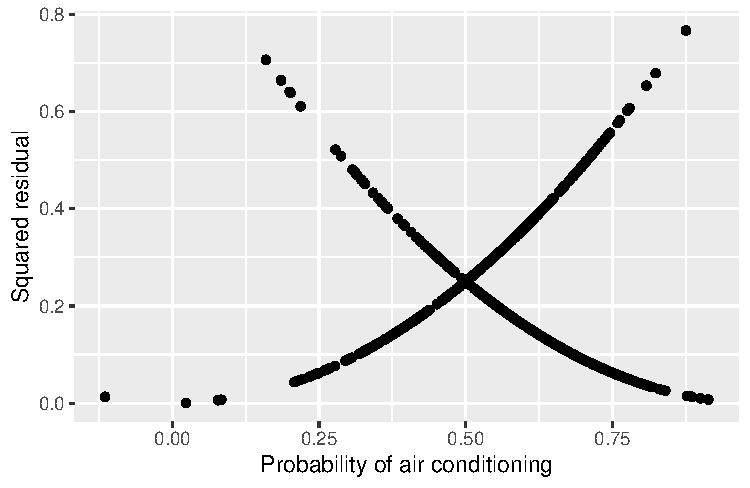
\includegraphics[width=\maxwidth]{figure/unnamed-chunk-16-1} 

}


\end{knitrout}
\end{frame}

\begin{frame}\frametitle{Cost Trade-Offs}
    How do consumers trade off the installation cost and the annual operating cost when choosing an HVAC system?
    \begin{itemize}
        \item What reduction in installation cost offsets a \$1 increase in the annual operating cost?
    \end{itemize}
    \begin{align*}
        U_{ni} & = \alpha_i + \beta_{1n} IC_{ni} + \beta_{2n} OC_{ni} + \varepsilon_{ni} \\
        dU_{ni} & = \beta_{1n} dIC_{ni} + \beta_{2n} dOC_{ni} \\
        dU_{ni} & = 0 ~~ \Rightarrow ~~ \frac{dIC_{ni}}{dOC_{ni}} = -\frac{\beta_{2n}}{\beta_{1n}}
    \end{align*}
    We do not know each decision maker's coefficients, but we do know the distribution of these individual-specific coefficients
    \begin{itemize}
    	\item We could find the distribution that corresponds to this ratio of distributions, but the ratio of normal distributions is challenging
    \end{itemize}
    \vspace{2ex}
    To make this question easier, we can estimate a model with a fixed $\beta_1$
\end{frame}

\begin{frame}[fragile]\frametitle{Mixed Logit Model with Random OC Coefficient}
    We model the utility of HVAC system $j$ to household $n$ as
    $$U_{nj} = \alpha_j + \beta_1 IC_{nj} + \beta_{2n} OC_{nj} + \varepsilon_{nj}$$
	  where the random coefficient is normally distributed
	  \begin{align*}
		  \beta_{2n} & \sim \mathcal{N}(\mu_2, \sigma_2^2)
	  \end{align*}
\begin{knitrout}\footnotesize
\definecolor{shadecolor}{rgb}{0.969, 0.969, 0.969}\color{fgcolor}\begin{kframe}
\begin{alltt}
\hlcom{## Model choice using alt intercepts and cost data with normal oc coef}
\hlstd{model_3} \hlkwb{<-} \hlkwd{mlogit}\hlstd{(}\hlkwc{formula} \hlstd{= depvar} \hlopt{~} \hlstd{ic} \hlopt{+} \hlstd{oc} \hlopt{|} \hlnum{1} \hlopt{|} \hlnum{0}\hlstd{,}
                  \hlkwc{data} \hlstd{= hvac_dfidx,}
                  \hlkwc{reflevel} \hlstd{=} \hlstr{'hpc'}\hlstd{,}
                  \hlkwc{rpar} \hlstd{=} \hlkwd{c}\hlstd{(}\hlkwc{oc} \hlstd{=} \hlstr{'n'}\hlstd{),}
                  \hlkwc{R} \hlstd{=} \hlnum{1000}\hlstd{,} \hlkwc{seed} \hlstd{=} \hlnum{703}\hlstd{)}
\end{alltt}
\end{kframe}
\end{knitrout}
\end{frame}

\begin{frame}[fragile]\frametitle{Mixed Logit Model Summary}
	  \vspace{1ex}
\begin{knitrout}\tiny
\definecolor{shadecolor}{rgb}{0.969, 0.969, 0.969}\color{fgcolor}\begin{kframe}
\begin{alltt}
\hlcom{## Summarize model results}
\hlkwd{summary}\hlstd{(model_3)}
\end{alltt}
\begin{verbatim}
## 
## Call:
## mlogit(formula = depvar ~ ic + oc | 1 | 0, data = hvac_dfidx, 
##     reflevel = "hpc", rpar = c(oc = "n"), R = 1000, seed = 703)
## 
## Frequencies of alternatives:choice
##   hpc    ec   ecc    er   erc    gc   gcc 
## 0.104 0.004 0.016 0.032 0.004 0.096 0.744 
## 
## bfgs method
## 9 iterations, 0h:0m:7s 
## g'(-H)^-1g = 2.15E-07 
## gradient close to zero 
## 
## Coefficients :
##                  Estimate Std. Error z-value  Pr(>|z|)    
## (Intercept):ec  -6.988571   1.777744 -3.9311 8.454e-05 ***
## (Intercept):ecc  1.989181   0.963761  2.0640 0.0390199 *  
## (Intercept):er  -9.033176   2.282496 -3.9576 7.571e-05 ***
## (Intercept):erc  0.719607   1.620491  0.4441 0.6569940    
## (Intercept):gc  -7.304331   2.161066 -3.3800 0.0007249 ***
## (Intercept):gcc  3.036280   0.477932  6.3530 2.112e-10 ***
## ic              -0.267513   0.081086 -3.2991 0.0009699 ***
## oc              -2.061273   0.486978 -4.2328 2.308e-05 ***
## sd.oc            0.535617   0.526907  1.0165 0.3093769    
## ---
## Signif. codes:  0 '***' 0.001 '**' 0.01 '*' 0.05 '.' 0.1 ' ' 1
## 
## Log-Likelihood: -198.12
## McFadden R^2:  0.12029 
## Likelihood ratio test : chisq = 54.18 (p.value = 1.0269e-11)
## 
## random coefficients
##    Min.   1st Qu.    Median      Mean   3rd Qu. Max.
## oc -Inf -2.422541 -2.061273 -2.061273 -1.700005  Inf
\end{verbatim}
\end{kframe}
\end{knitrout}
\end{frame}

\begin{frame}[fragile]\frametitle{Interpreting Parameters}
\begin{knitrout}\footnotesize
\definecolor{shadecolor}{rgb}{0.969, 0.969, 0.969}\color{fgcolor}\begin{kframe}
\begin{alltt}
\hlcom{## Display model coefficients}
\hlkwd{coef}\hlstd{(model_3)}
\end{alltt}
\begin{verbatim}
##  (Intercept):ec (Intercept):ecc  (Intercept):er (Intercept):erc 
##      -6.9885711       1.9891815      -9.0331761       0.7196068 
##  (Intercept):gc (Intercept):gcc              ic              oc 
##      -7.3043311       3.0362800      -0.2675133      -2.0612730 
##           sd.oc 
##       0.5356169
\end{verbatim}
\end{kframe}
\end{knitrout}
    \vspace{2ex}
    How do we interpret these coefficients?
    \begin{itemize}
    	\item Alternative-specific intercepts
    	\begin{itemize}
    		\item \texttt{ecc} and \texttt{gcc} provide more utility, \emph{ceteris paribus}, than \texttt{hpc}
	        \item \texttt{erc} provides the same utility, \emph{ceteris paribus}, as \texttt{hpc}
	        \item \texttt{ec}, \texttt{er}, and \texttt{gc} provide less utility, \emph{ceteris paribus}, than \texttt{hpc}
    	\end{itemize}
        \item An additional \$100 of installation cost reduces utility by 0.27
        \item An additional \$100 of annual operating cost reduces utility by 2.06 on average with a standard deviation of 0.54
    \end{itemize}
\end{frame}

\begin{frame}[fragile]\frametitle{Test of Random Coefficient Variance}
	We just estimated a model that restricted $\beta_1$ to be fixed, which is equivalent to saying $\beta_1$ is random with zero variance, or $\sigma_1^2 = 0$
	\begin{itemize}
		\item We can test if this imposed restriction is correct
	\end{itemize}
    \vspace{3ex}
    We will test the null hypothesis
    $$H_0 \text{: } \sigma_1^2 = 0$$ \\
\begin{knitrout}\footnotesize
\definecolor{shadecolor}{rgb}{0.969, 0.969, 0.969}\color{fgcolor}\begin{kframe}
\begin{alltt}
\hlcom{## Conduct likelihood ratio test of models 2 and 3}
\hlkwd{lrtest}\hlstd{(model_2, model_3)}
\end{alltt}
\begin{verbatim}
## Likelihood ratio test
## 
## Model 1: depvar ~ ic + oc | 1 | 0
## Model 2: depvar ~ ic + oc | 1 | 0
##   #Df  LogLik Df  Chisq Pr(>Chisq)    
## 1  10 -192.14                         
## 2   9 -198.12 -1 11.958  0.0005443 ***
## ---
## Signif. codes:  0 '***' 0.001 '**' 0.01 '*' 0.05 '.' 0.1 ' ' 1
\end{verbatim}
\end{kframe}
\end{knitrout}
\end{frame}

\begin{frame}[fragile]\frametitle{Cost Trade-Offs}
    How do consumers trade off the installation cost and the annual operating cost when choosing an HVAC system?
    \begin{itemize}
        \item What reduction in installation cost offsets a \$1 increase in the annual operating cost?
    \end{itemize}
    $$\frac{dIC_{ni}}{dOC_{ni}} = -\frac{\beta_{2n}}{\beta_1}$$ \\
    Because $\beta_{2n}$ is normally distributed and  $\beta_1$ is fixed, the ratio is also a normal distribution
    $$\frac{dIC_{ni}}{dOC_{ni}} \sim \mathcal{N} \left( \frac{\mu_2}{\beta_1}, \frac{\sigma_2^2}{\beta_1^2} \right)$$
    \begin{itemize}
    	\item What are the mean and standard deviation of this distribution?
    \end{itemize}
\begin{knitrout}\footnotesize
\definecolor{shadecolor}{rgb}{0.969, 0.969, 0.969}\color{fgcolor}\begin{kframe}
\begin{alltt}
\hlcom{## Calculate ic equivalence of an increase in oc}
\hlkwd{c}\hlstd{(}\hlopt{-}\hlkwd{coef}\hlstd{(model_3)[}\hlnum{8}\hlstd{]} \hlopt{/} \hlkwd{coef}\hlstd{(model_3)[}\hlnum{7}\hlstd{],}
  \hlkwd{abs}\hlstd{(}\hlkwd{coef}\hlstd{(model_3)[}\hlnum{9}\hlstd{]} \hlopt{/} \hlkwd{coef}\hlstd{(model_3)[}\hlnum{7}\hlstd{]))}
\end{alltt}
\begin{verbatim}
##        oc     sd.oc 
## -7.705311  2.002207
\end{verbatim}
\end{kframe}
\end{knitrout}
\end{frame}

\begin{frame}[fragile]\frametitle{Plot of Cost Trade-offs}
\begin{knitrout}\footnotesize
\definecolor{shadecolor}{rgb}{0.969, 0.969, 0.969}\color{fgcolor}\begin{kframe}
\begin{alltt}
\hlcom{## Plot distributions of random coefficients}
\hlkwd{ggplot}\hlstd{(}\hlkwc{data} \hlstd{=} \hlkwd{data.frame}\hlstd{(}\hlkwc{x} \hlstd{=} \hlkwd{c}\hlstd{(}\hlopt{-}\hlnum{18}\hlstd{,} \hlnum{2}\hlstd{)),} \hlkwd{aes}\hlstd{(x))} \hlopt{+}
  \hlkwd{stat_function}\hlstd{(}\hlkwc{fun} \hlstd{= dnorm,} \hlkwc{n} \hlstd{=} \hlnum{1001}\hlstd{,}
                \hlkwc{args} \hlstd{=} \hlkwd{list}\hlstd{(}\hlkwc{mean} \hlstd{=} \hlopt{-}\hlkwd{coef}\hlstd{(model_3)[}\hlnum{8}\hlstd{]} \hlopt{/} \hlkwd{coef}\hlstd{(model_3)[}\hlnum{7}\hlstd{],}
                            \hlkwc{sd} \hlstd{=} \hlkwd{abs}\hlstd{(}\hlkwd{coef}\hlstd{(model_3)[}\hlnum{9}\hlstd{]} \hlopt{/}
                                       \hlkwd{coef}\hlstd{(model_3)[}\hlnum{7}\hlstd{])))} \hlopt{+}
  \hlkwd{xlab}\hlstd{(}\hlkwa{NULL}\hlstd{)} \hlopt{+}
  \hlkwd{ylab}\hlstd{(}\hlkwa{NULL}\hlstd{)}
\end{alltt}
\end{kframe}
\end{knitrout}
\end{frame}

\begin{frame}[fragile]\frametitle{Plot of Cost Trade-offs}
\begin{knitrout}\footnotesize
\definecolor{shadecolor}{rgb}{0.969, 0.969, 0.969}\color{fgcolor}

{\centering \includegraphics[width=\maxwidth]{figure/unnamed-chunk-23-1} 

}


\end{knitrout}
\end{frame}

\end{document}
